% !TEX root = ../ClassicThesis_DEIB.tex

\chapter{The Robì project} \label{chap:robìProject}

A branch of this thesis work involved the customization of the prototype mobile manipulator Robì \parencite{robi} to the requirements of the mobile base requested by the \ac{GRAPE} project. 


\begin{figure}
	\centering
	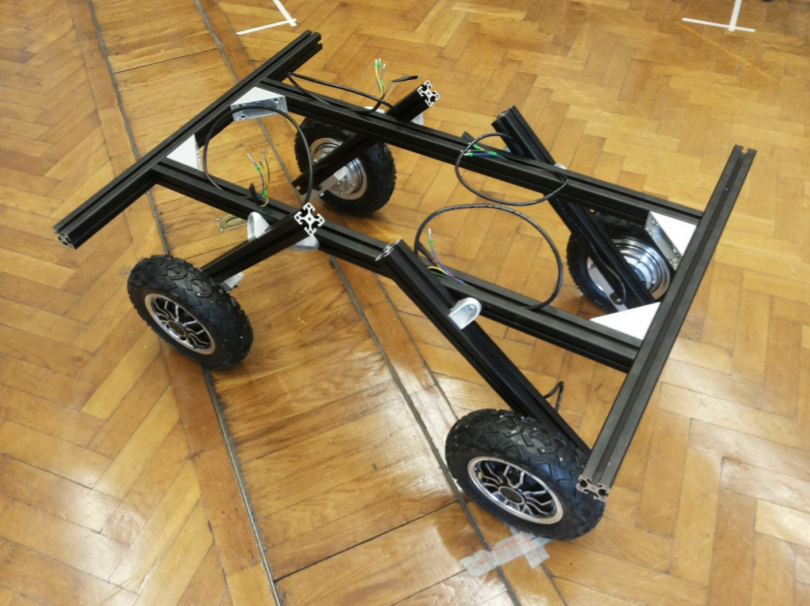
\includegraphics[width=0.6\textwidth]{Images/robi/robi_inizio.png}
	\caption{\textit{The Robì mobile manipulator chassis, in one of its}}
	\label{fig:robiDefault}
\end{figure}


\section{Robì mobile manipulator}\label{sec:robiDescr}
Robì (see Figure \ref{fig:robiDefault}) is a prototype small-sized mobile manipulator for agricultural applications, whose aim is to support the development and testing of innovative perception and control algorithms. Both the mechanical structure and the motion control system are designed to be simple, flexible, low-cost and low-weight, to create a system that can act as an open source base for project in agricultural robotics, contrary to the large amount of task-specific platforms in agricultural robotics (\textit{e.g.} for asparagus \parencite{asparagi} or tomato \parencite{pomodori} harvesting).

\par Since the platform is thought as a versatile mobile base to be adapted to several fields (\textit{e.g.} vineyards, herbaceous plants) its chassis is designed to have flexible geometrical characteristics (ground clearance, track, wheelbase).

 \begin{table}[tb]
\footnotesize
\centering
\begin{tabularx}{0.45\textwidth}{ll}
\toprule
\tablefirstcol{l}{Ground clearance}
& [0.25, 0.35] m \\
\tablefirstcol{l}{Track}
& [0.75, 1.2] m \\
\tablefirstcol{l}{Wheelbase}
& [0.6, 1] m \\
\toprule
\end{tabularx}
\caption[Ranges of Robì geometrical characteristics]{\textit{Ranges of Robì geometrical characteristics.}}
\label{tab:robiConfiguration}
\end{table}

 More generally, the design principles of Robì are:
 
\begin{itemize}
	\item \textbf{low cost}, to make it easier to use it for example applications and, possibly, fleet-based applications
	\item \textbf{low weight}, to increase the battery life and, consequently, allow for more long and versatile missions
	\item \textbf{simple mechanical design}, to make it easy to build it out of a mounting kit
\end{itemize}

\begin{figure}
	\centering
	\subfloat[]{%
		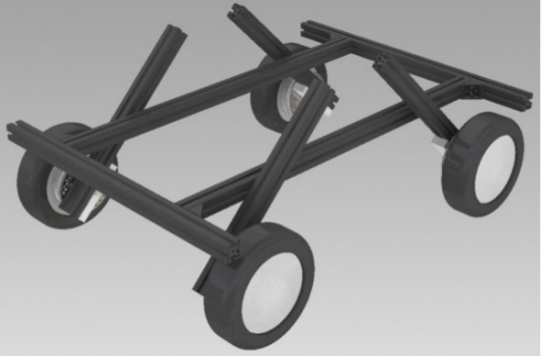
\includegraphics[width=0.45\textwidth]{Images/robi/robi_config1.png}
		\label{fig:robiConfig1}}
	\qquad
	\subfloat[]{%
		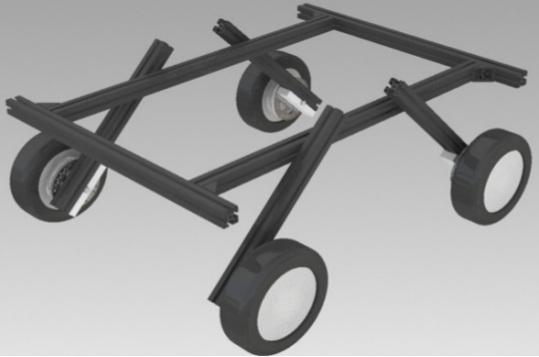
\includegraphics[width=0.45\textwidth]{Images/robi/robi_config2.png}
		\label{fig:robiConfig2}} \\
	\subfloat[]{%
		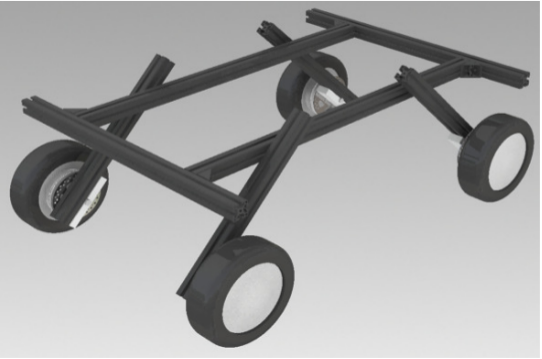
\includegraphics[width=0.45\textwidth]{Images/robi/robi_config3.png}
		\label{fig:robiConfig3}}
	\caption{\textit{3D rendering of different configuration of Robì base, obtained thanks to the chassis mechanical design.}}
	\label{fig:robiConfigurations}
\end{figure}

The aforementioned principles are implemented through the following design choices:
\begin{description}
	\item[Chassis] \hfill \\ The chassis is made out of ITEM\textsuperscript{\textregistered} aluminium bars, that presents lightweight but strong section; the slide rails embedded in the ITEM\textsuperscript{\textregistered} bars, together with four rotational joints applied to the bars supporting the wheels, allow for multiple configuration of the robot geometrical characteristics to vary in the ranges listed in Table \ref{tab:robiConfiguration}. In Figure \ref{fig:robiConfigurations} you can see 3D rendering of some of the available Robì configurations. The bars that support the wheel, however, can't rotate during the robot movement, thus Robì has a skid steering kinematic model.
	
	\item[In-wheel motors] \hfill \\ Robì is powered by four in-wheel electric DC brushless motors; the model is HUB10GL (see Figure \ref{fig:robiMotori}). In-wheel motors have been chosen mostly because they allow for much simpler mechanical design, with respect to classical electrical powertrain, because:
	\begin{itemize}
		\item no transmission is required
		\item the weight is reduced, and the available space on the chassis increases
		\item high level of maneuverability, without the need to introduce Ackermann kinematics
	\end{itemize}
	The motors are independent, so a suitable control board is required to control each of them; the board used in Robì are the ones described in VESC project\footnote{\url{http://vedder.se/2015/01/vesc-open-source-esc/}},
an open source brushless motor control project. These boards offers several interfaces to control the motor:  PPM signal, analog, UART, I$^2$C, USB  or CAN-bus.
\end{description}

\begin{figure}
	\centering
	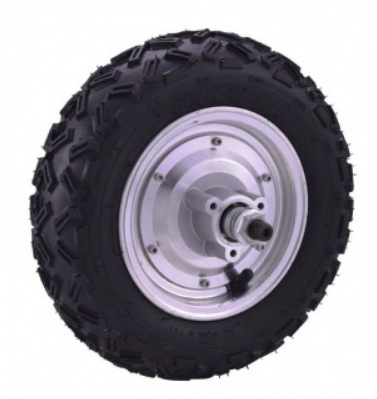
\includegraphics[width=0.4\textwidth]{Images/robi/motore.png}
	\caption{\textit{HUB10GL, the in-wheel motor model adopted in Robì.}}
	\label{fig:robiMotori}
\end{figure}

\section{Robì as GRAPE robotic base}
The features mentioned in the previous section made Robì a convincing candidate as the mobile platform for the \ac{GRAPE} project, because of its flexibility as a mobile manipulator for agricultural robotics field. Unfortunately, for mere lack of time, in the late phases the project focused on the development of the whole system on a commercial robot, the Husky that was already described as the final \ac{UGV} of the \ac{GRAPE} project.
\par However, significant steps in the adaptation of Robì as a base for a real agricultural robotic project were made, thus we are explaining them in this section.

\subsection{Hardware configuration}
Since our goal was to create the system that was later developed on the Husky robot, the sensor mounted on it were similar; on the other side, we had to dedicate significant efforts to the creation of an hardware interface between the on-board computer (a commercial HP laptop) and the motors control boards. Given the flexibility of Robì physical structure, we decided to add a simple structure in the frontal part of Robì as a support for the bulkier sensors (see Figure \ref{fig:robiGrape}), built out of ITEM\textsuperscript{\textregistered} for compatibility. Note that the Jaco$^2$ was still the designated arm in this configuration (see Figure \ref{fig:grapeRobiWithArm}).
\begin{description}


\begin{figure}
	\centering
	\subfloat[]{%
		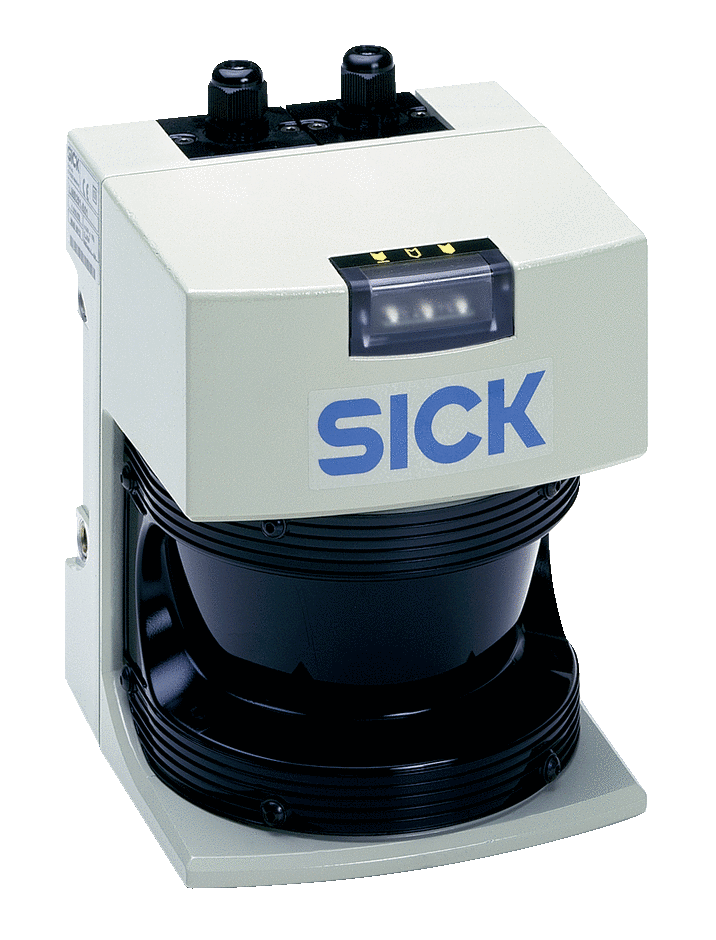
\includegraphics[width=0.3\textwidth]{Images/robi/lidar_singlerange.png}
		\label{fig:lms291}}
	\qquad
	\subfloat[]{%
		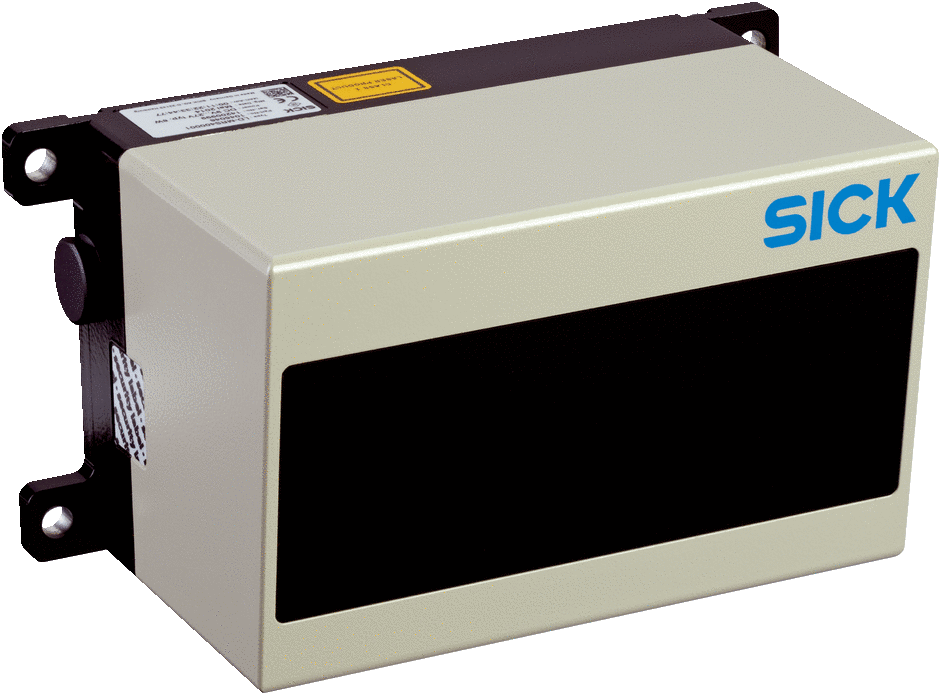
\includegraphics[width=0.3\textwidth]{Images/robi/lidar_multirange.png}
		\label{fig:LD-MRS400001}}
	\subfloat[]{%
		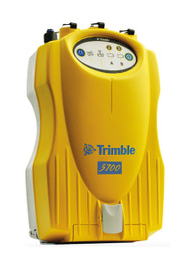
\includegraphics[width=0.3\textwidth]{Images/robi/trimble5700.png}
		\label{fig:trimble5700}}
	\caption{\textit{Some of the sensors Robì is equipped with: LMS291 (\ref{fig:lms291}), and LD-MRS400001 (\ref{fig:LD-MRS400001}), both laser scanners from SICK; Trimble 5700 GPS transceiver (\ref{fig:trimble5700}), from Trimble}}
\end{figure}

	\item[LIDARS] \hfill \\ In section \ref{sec:robiDescr} we pointed out that Robì, as the Husky robot, comes up with a skid steering kinematic model. Thus, we chose to use two frontal \ac{LIDAR}s for obstacles avoidance during navigation tasks. The \ac{LIDAR} models were:
	\begin{itemize}
		\item \textbf{Sick LMS291}: this sensor\footnote{\url{https://www.sick.com/ag/en/detection-and-ranging-solutions/2d-lidar-sensors/lms2xx/lms291-s05/p/p109849}}
		only has a single measuring plane, maintained parallel to the ground, in order to detect long-range obstacles during navigation tasks
		\item \textbf{Sick LD-MRS400001}: this sensor\footnote{\url{https://www.sick.com/de/en/detection-and-ranging-solutions/3d-lidar-sensors/ld-mrs/ld-mrs400001/p/p112355}}
		is a multi-range laser scanner, with 4 measuring planes with narrow aperture angles. Unlike \textit{LMS291} scanner, its arrangement in the sensors support bar is slightly tilted forward, to be able to scan closer obstacles.
	\end{itemize}
	
\begin{table}[tb]
\footnotesize
\centering
\begin{tabularx}{0.75\textwidth}{lll}
\toprule
\tableheadline{l}{}  &
\tableheadline{r}{LMS291}  &
\tableheadline{r}{LD-MRS400001}  \\
\midrule
\tablefirstcol{l}{Number of Channels}
&1  &4 \\
\midrule
\tablefirstcol{l}{Scan Angle}
&180°  & 85°\\
\midrule
\tablefirstcol{l}{Rotation rate}
&75Hz    & 12.5 Hz \\
\midrule
\tablefirstcol{l}{Angular Resolution}
& 0.25° & 0.125° \\
\midrule
\tablefirstcol{l}{Range}
&80m  & 300m \\
\midrule
\tablefirstcol{l}{Power Consumption}
&30W  & 8W \\
\midrule
\tablefirstcol{l}{Weight}
&4.5kg & 1kg \\
\bottomrule
\end{tabularx}
\caption[Robì \ac{LIDAR}s comparison]{Comparison of Robì on-board \ac{LIDAR}s}
\label{tab:robiLidarComparison}
\end{table}
	
	\item[GPS] \hfill \\ We opted for a very reliable solution, the \textbf{Trimbe 5700} GPS receiver (see Figure \ref{fig:trimble5700}) from Trimble, together with its dedicated antenna. 
	
	\item[RADIO] \hfill \\ In order to easily control and monitor the activity of the \ac{UGV} especially during outdoor tasks, we also installed on Robì the required hardware to create a \textit{point-to-point} radio bridge with another base station (\textit{e.g.} another laptop in a more comfortable place). Two base stations were chosen, which performance were measured in urban environment (because, as already stated, the development of Robì as \ac{GRAPE} robotic base was aborted before \textit{on-the-field} validation):
	\begin{itemize}
		\item \textbf{Rocket M5} station\footnote{\url{https://dl.ubnt.com/datasheets/rocketm/RocketM_DS.pdf}}
		from Ubiquiti, together with an omni-directional antenna, mounted directly on Robì
		\item \textbf{NanoStation M5} station\footnote{\url{https://dl.ubnt.com/datasheets/nanostationm/nsm_ds_web.pdf}}
		from Ubiquiti, to be used from the control device.
	\end{itemize}
	This couple of devices were able to durably create a radio link of \textasciitilde340 meters.
	
	\item[Motors interface] \hfill \\ In order to communicate with the motors control boards, we had to introduce a single hardware interface among them and the on-board PC. We decided to use \textbf{NUCLEO-F746ZG} development board\footnote{\url{http://www.st.com/en/evaluation-tools/nucleo-f746zg.html}}
	from ST (see Figure \ref{fig:nucleoBoardAlone}). It provides:
	\begin{itemize}
		\item RJ-45 Ethernet interface, very useful to communicate with the on-board PC
		\item CAN protocol interface, to communicate with the motors control boards
		\item ST Zio connector, which extends the Arduino Uno V3 connectivity and provides an easy means of expanding the functionality of the Nucleo platform with a wide choice of specialized shields
	\end{itemize}
	In particular, the interface with the on-board PC was implemented as a bidirectional UDP connection. This will be cleared out in Section \ref{sec:robiSoftware}.
	
\begin{figure}
	\begin{minipage}[c]{.5\textwidth}
	\centering	
	\subfloat[]{%
		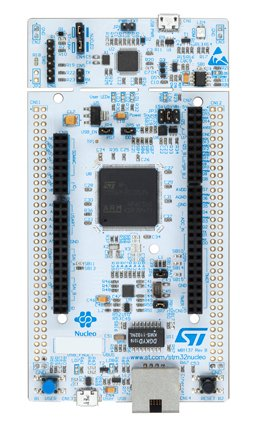
\includegraphics[width=0.55\textwidth]{Images/robi/nucleoBoard.jpg}
		\label{fig:nucleoBoardAlone}}
	\end{minipage}
	\begin{minipage}[c]{.5\textwidth}
	\subfloat[]{%
		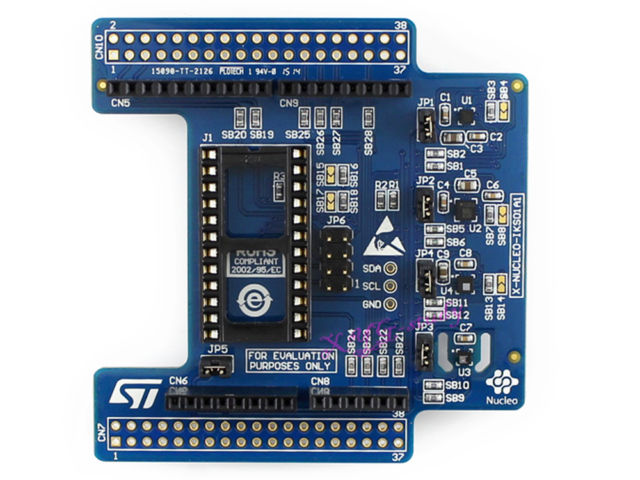
\includegraphics[width=0.8\textwidth]{Images/robi/shield.jpg}
		\label{fig:imuShield}}
	\end{minipage}
	\caption{\textit{The Nucleo board we used to communicate with the motors control board (Figure \ref{fig:nucleoBoardAlone}), and the shield mounted on it to integrate \ac{IMU} sensor (see Figure \ref{fig:imuShield}).}}
	\label{fig:nucleoBoard}
\end{figure}

	\item[IMU] \hfill \\ For the choice of \ac{IMU}, we decided to take advantage of the Zio interface of the Nucleo board, so we inserted in the system the \textbf{x nucleo iks01a1} shield\footnote{\url{http://www.st.com/en/ecosystems/x-nucleo-iks01a1.html}}
	(see Figure \ref{fig:imuShield}).
	This shield includes:
	\begin{itemize}
		\item LSM6DS0 MEMS 3D accelerometer and 3D gyroscope
		\item LIS3MDL MEMS 3D magnetometer
	\end{itemize}
\end{description}



\begin{figure}
	\centering
	\subfloat[]{%
		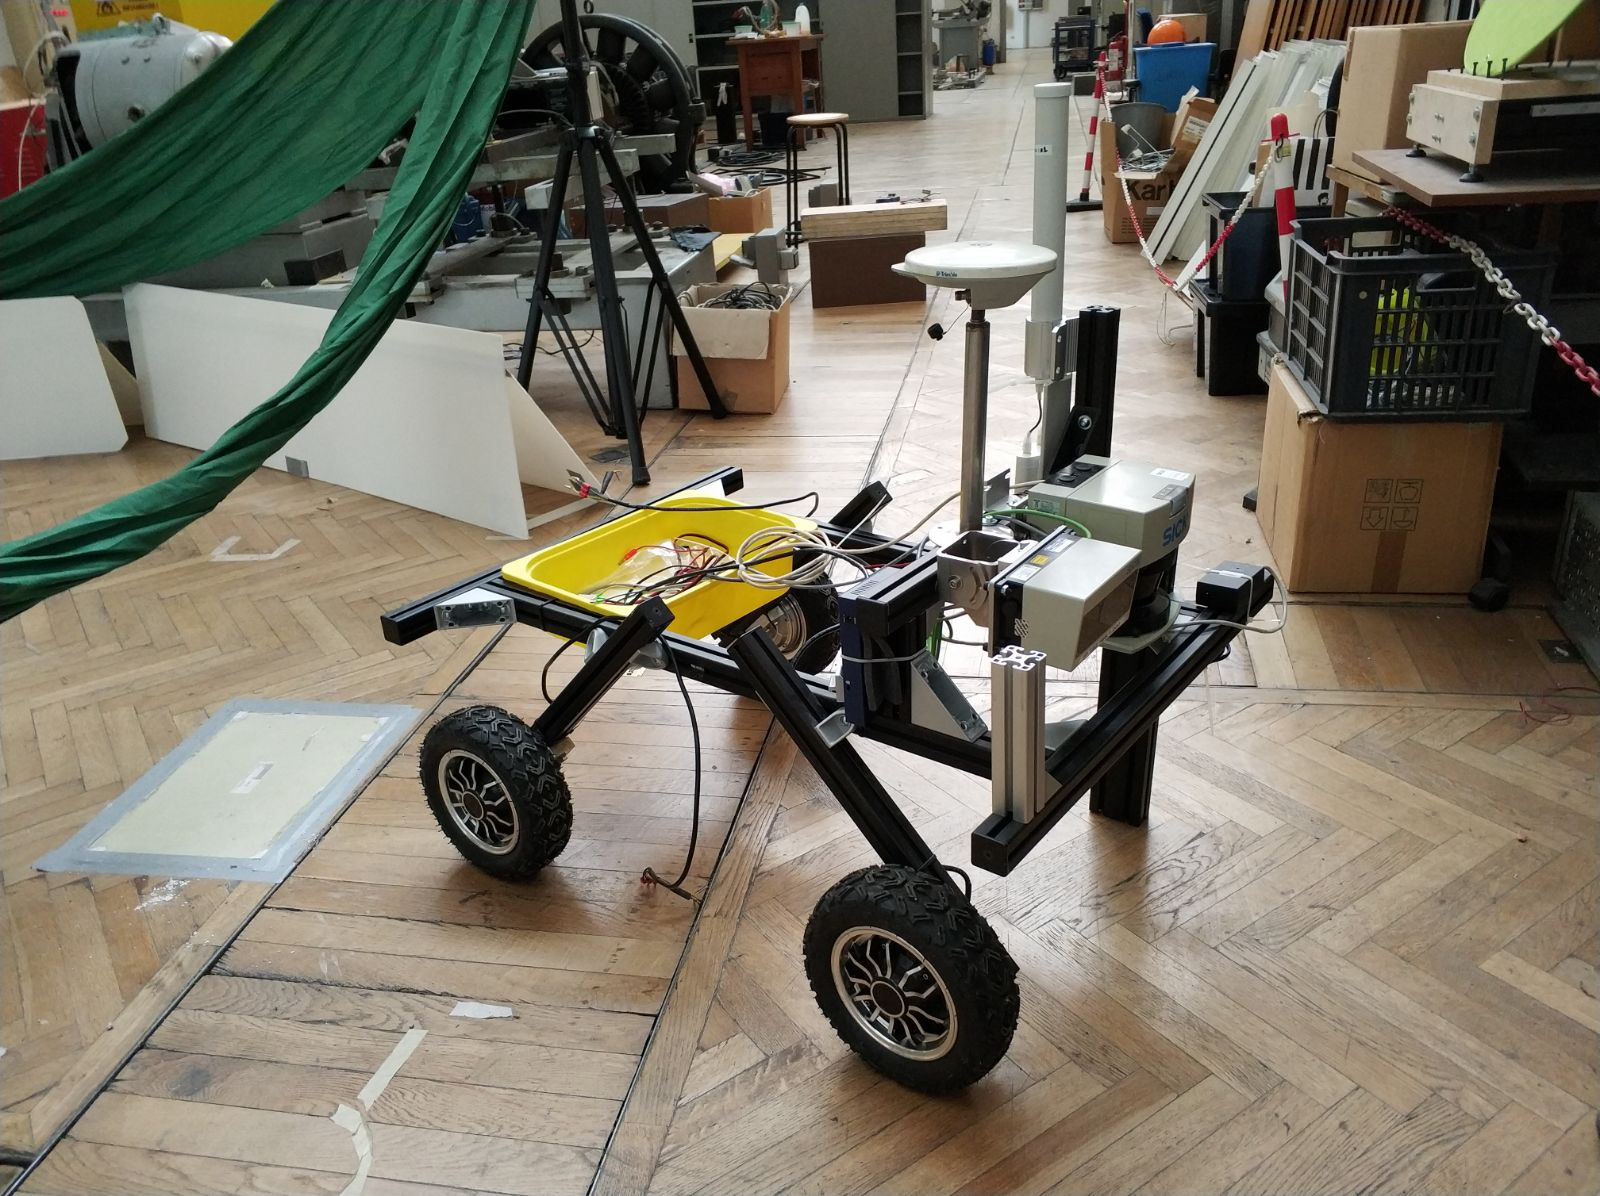
\includegraphics[width=0.5\textwidth]{Images/robi/robiGrapeNoArm.jpeg}
		\label{fig:grapeRobiNoArm}}
	\qquad
	\subfloat[]{%
		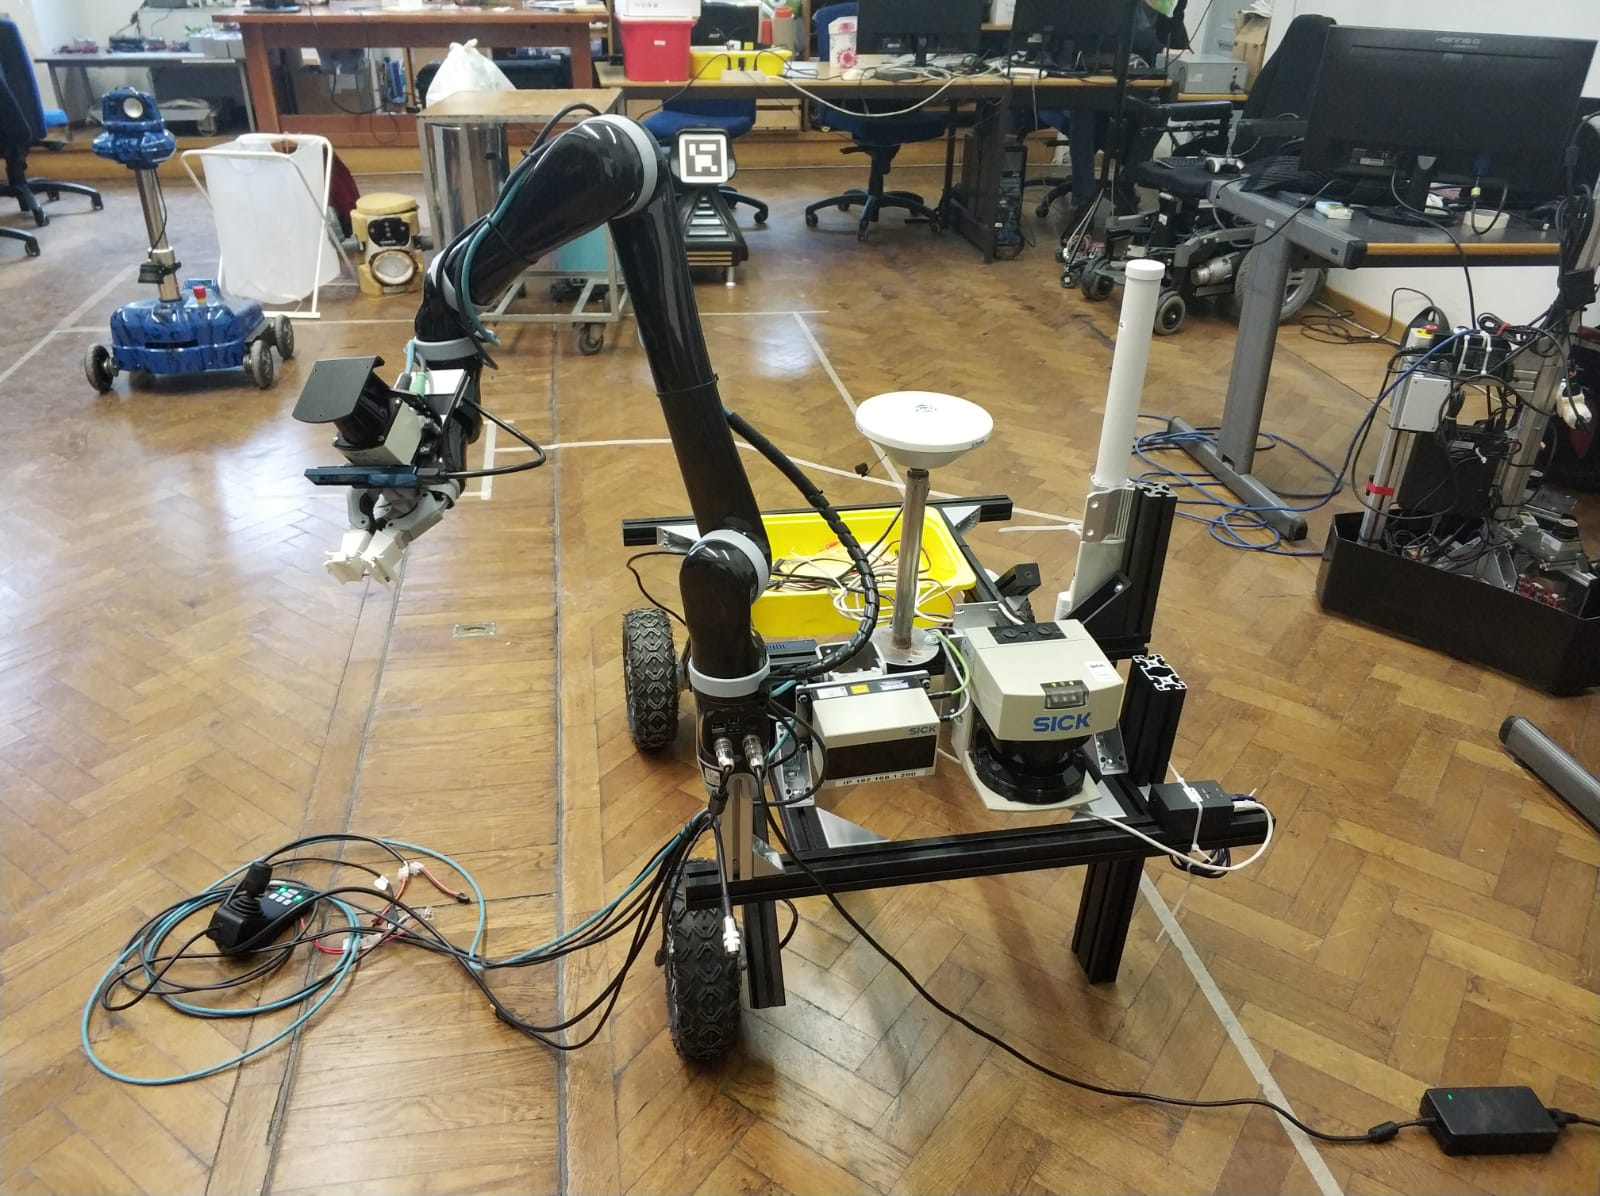
\includegraphics[width=0.5\textwidth]{Images/robi/robiGrapeWithArm.jpeg}
		\label{fig:grapeRobiWithArm}}
	\caption{\textit{3D rendering of different configuration of Robì base, obtained thanks to the chassis mechanical design.}}
	\label{fig:robiGrape}
\end{figure}


\begin{itemize}
	\item architettura hw: sensori che ci sono montati a bordo, spiegazione sistema controllo motori tramite CAN usando la board STM
	\item architettura sw: compatibile con quella di Grape, a meno dei nodi driver dei sensori e attuatori
	\item spiegazioni e immagini del vario hardware
\end{itemize}
